\documentclass[a4paper,12pt]{report}
\usepackage[utf8]{inputenc}
\usepackage{amsmath}
\usepackage{graphicx}
\usepackage{listings}
\usepackage{tikz}
\usepackage[T1]{fontenc}
\usepackage{color}
\usetikzlibrary{arrows,automata}
\definecolor{pythonred}{rgb}{0.6,0,0} % for strings
\definecolor{pythongreen}{rgb}{0.25,0.5,0.35} % comments
\definecolor{pythonpurple}{rgb}{0.5,0,0.35} % keywords
	\definecolor{pythondocblue}{rgb}{0.25,0.35,0.75} % javadoc
	 
	\lstset{language=python,
	basicstyle=\ttfamily,
	keywordstyle=\color{pythonpurple}\bfseries,
	stringstyle=\color{pythonred},
	commentstyle=\color{pythongreen},
	morecomment=[s][\color{pythondocblue}]{/**}{*/},
	numbers=left,
	numberstyle=\tiny\color{black},
        stepnumber=2,
	numbersep=10pt,
	tabsize=4,
	showspaces=false,
	showstringspaces=false}

% Title Page

 \title{\bfseries\huge \textcolor{purple}{\underline {EEP-703 Computer Network Lab}} \\{\textcolor{blue}{Assignment5-Simulate classical queueing models like M/M/1 in NS2}}}
\author{\bfseries\large\textcolor{black}  {Harshit Kumar Gupta}\\ {\textcolor{black} {2013EET2369 }}\\

\includegraphics[width=3cm,height=3.4cm]{./iit.png}\\\noindent Computer Technology\\
\noindent Department Of Electrical Engineering\\IIT DELHI}
% iit.png: 282x282 pixel, 72dpi, 9.95x9.95 cm, bb=0 0 282 282
\begin{document}
\maketitle
\tableofcontents


\chapter{\textcolor{blue}{\underline {PROBLEM STATEMENT}}}
\noindent 

         Consider a mail server of IIT Delhi with three departments have separate mail servers along
with an external mail server. The external mail server receives mails from all the three
department mail servers. Label the main server as node 0 and other three servers as node 1, 2
and 3. The messages, each with mean arrival rate 30 messages/sec arrive from three
department servers. The capacity of each duplex link is 100kb/sec with 5ms delay. Simulate
for 5 minutes to get the following performance measures. (consider M/M/1 queue between
the transmitting and the receiving nodes )

	
	\begin{enumerate}
	  \item Throughput at the central server (plot throughput versus simulation time).
	  \item  Plot queue length vs time and also calculate average queue length. (use monitor-queue
                 trace called qm.out)
	\end{enumerate}
	\noindent Compare the throughput at the central server when the queue size for all the links are changed
to 500 with that of default queue size provided in NS2. Give an explanation of the results
obtained. (M/M/1/K i.e. limited queue size)\\
	\noindent Simulate the above given scenario for M/D/1 queueing model.

\begin{center}
\chapter{\textcolor{blue}{\underline {ABSTRACT}}}
\end{center}
\noindent The entire code has been written as to simulate on a Network Simulator which inputs a 'tcl' file and when compiled with a ns2 Simulator generates a 'trace' file as Output.
	  Furthermore awk script has been used as to clip out the columns of the trace file and to act them as parameters for deciding the effect of bottlenecks in the Network through
	  realising the Packet Size and the inter delay time between the packets. Finally the value of those parameters is plotted using the 'gnuplot' tool so as to show the result in a graph.
\begin{center}
\chapter{\textcolor{blue}{\underline {INTRODUCTION}}}
\end{center}
\noindent \textbf In 1996-97, ns version 2 (ns-2) was initiated based on a refactoring by Steve McCanne. Use of Tcl was replaced by MIT's Object Tcl (OTcl), an object-oriented dialect of Tcl.
		  The core of ns-2 is also written in C++, but the C++ simulation objects are linked to shadow objects in OTcl and variables can be linked between both language realms.
		  Simulation scripts are written in the OTcl language, an extension of the Tcl scripting language.
                  Presently, ns-2 consists of over 300,000 lines of source code, and there is probably a comparable amount of contributed code that is not integrated directly into the main distribution of ns-2 exist,
                  both maintained and unmaintained. It runs on GNU/Linux, FreeBSD, Solaris, and Mac OS X.\\
		  
		  AWK is an interpreted programming language designed for text processing and typically used as a data extraction and reporting tool. 
		  It is a standard feature of most Unix-like operating systems. AWK was very popular in the late 1970s and 1980s, but from the 1990s has largely been replaced by Perl,
		  on which AWK had a strong influence.\\
		  
		 While the gnuplot is a command-line program that can generate two- and three-dimensional plots of functions, data, and data fits. 
		    It is frequently used for publication-quality graphics as well as education.gnuplot can produce output directly on screen, 
		    or in many formats of graphics files, including Portable Network Graphics (PNG), Encapsulated PostScript (EPS), Scalable Vector Graphics (SVG), JPEG and many others. 
		    It is also capable of producing LaTeX code that can be included directly in LaTeX documents, making use of LaTeX's fonts and powerful formula notation abilities.
		    The program can be used both interactively and in batch mode using scripts.

\begin{center}
\chapter{\textcolor{blue}{\underline {SPECIFICATIONS AND ASSUMPTIONS}}}
\end{center}
\section*{Specifications}
\begin{enumerate}
 

 \item M/M/1 Queue and M/M/1-K Queue are used as queueing models
 \item Constant bit rate to be taken is 100kbps and lamda=30, mue=33.
 \item Perfomance Comparison has to be done with the help of THROUGHPUT.
\end{enumerate}

\section*{Assumptions}
\begin{enumerate}
\item ns2 Simulator will be used for compiling the tcl file.
\item Inspite of perl ; 'awk' tool will be used to cut the parameters.
\item 'gnuplot' has been used to plot the values of Throughput.
\item For nodes the Z coordinate is assumed to be '0'
\item Other throughput degradation factors have been ignored.
\end{enumerate}
 
\begin{center}
\chapter{\textcolor{blue}{\underline {LOGIC USED/METHODOLOGY}}}
\end{center}
The methodology that is used for developing this project work is defined below:
\begin{enumerate} 
\item The entire code is written in tcl file format.
\item First, all the required 4 nodes are created in which node 0 acts as main server and node 1, 2, 3 are the departmental servers.
\item All the nodes 1, 2, 3 sends data to main server node 0.
\item A UDP connection is set up between nodes 1, 2, 3 and node 0.
\item Once the file is compiled it , the Output trace file is generated.
\item After the Trace file is generated it has to be compiled with the 'awk' file.
\item For Calculating the Throughput and queue length versus time graph, awk file is created as per the Formulae and Appropriate Variable Assumptions in the Trace File.
\item Finally gnuplot Tool is used to make two separate Graphs for M/M/1 and M/M/1-K queueing model on Network Behaviour.
\end{enumerate}


\begin{center}
\chapter{\textcolor{blue}{\underline {Execution Directives}}}
\end{center}
\noindent \\ In the terminal of LINUX system the following commands are executed in order to create a network topology and its analysis.\\
\begin{enumerate}
\item ns mm1.tcl
\item awk -f file.awk qm1.out > qm1.data
\item awk -f file.awk qm2.out > qm2.data
\item awk -f file.awk qm3.out > qm3.data
\item aek -f awk_script mm1.tcl >parameters.dat
\item gnuplot queueLength.plot
\item gnuplot throughput.plot
\item gnuplot interarrival.plot

\end{enumerate}
\noindent Repeat the above procedures for M/M/1 queue modeling and also for static router condition as mentioned in the problem statement.

\begin{center}
\chapter{\textcolor{blue}{\underline {PLOTS And FIGURES}}}
\end{center}
\noindent Fig-1: Topology Designed in Network Simulator.\\
\begin{center}
 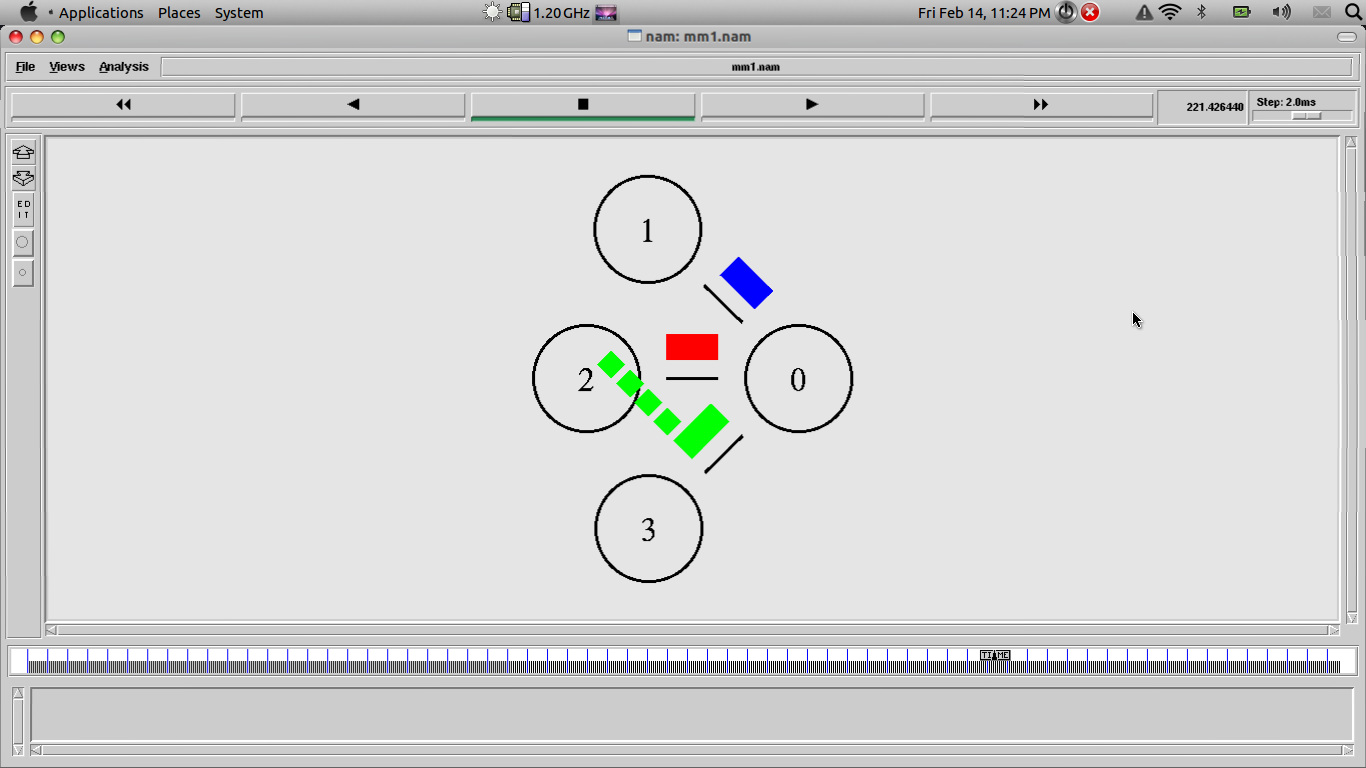
\includegraphics[width=13 cm,height=13 cm]{./Screenshot.png}
 % protocol.png: 1280x800 pixel, 72dpi, 45.16x28.22 cm, bb=0 0 1280 800
\end{center}


\noindent Fig-2: Throughput Vs Time Graph(for M/M/1 model )\\
\begin{center}
 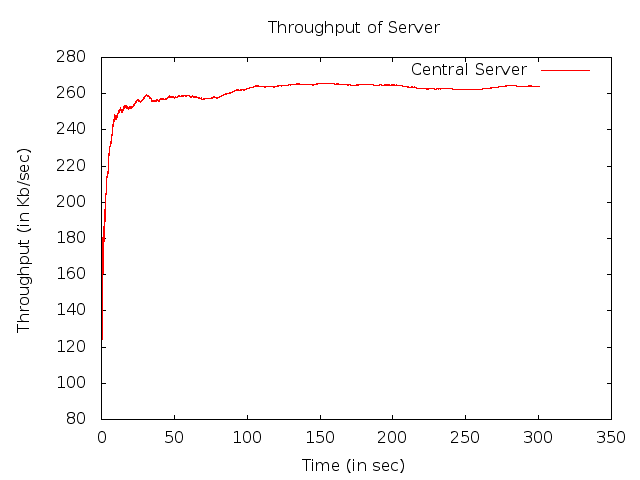
\includegraphics[width=12 cm,height=12 cm]{../problem/throughput.png}
 % Throughput.png: 640x480 pixel, 72dpi, 22.58x16.93 cm, bb=0 0 640 480
\end{center}

\noindent Fig-3: Queue Length Vs Time Graph(for M/M/1 model )\\
\begin{center}
 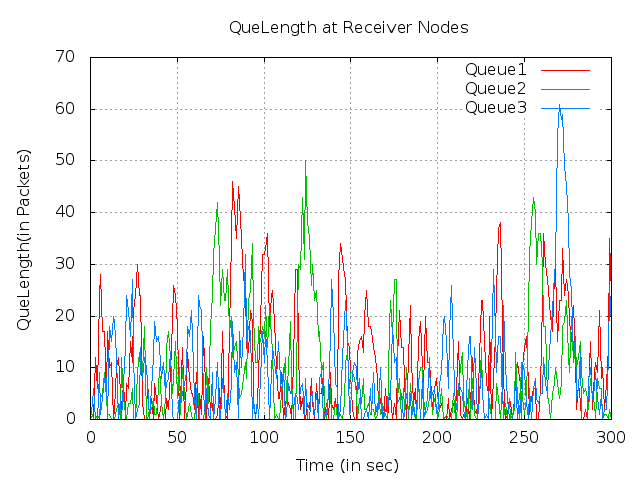
\includegraphics[width=12 cm,height=12 cm]{../problem/queuelength.png}
 % queuelength.png: 640x480 pixel, 72dpi, 22.58x16.93 cm, bb=0 0 640 480
\end{center}
\noindent Fig-4: Interarrival Time Vs Time Graph(for M/M/1 model )\\
\begin{center}
 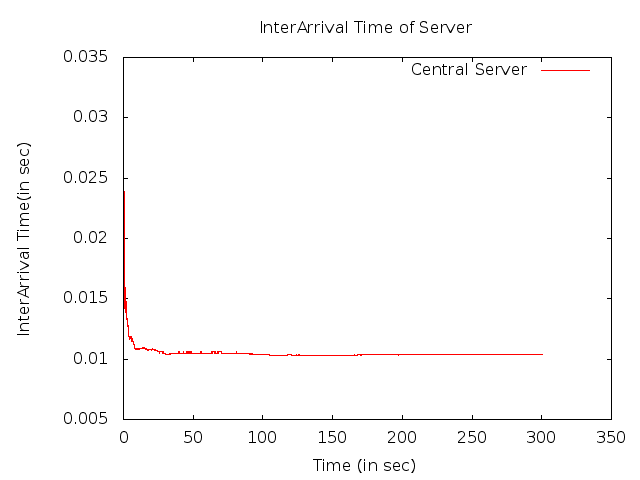
\includegraphics[width=12 cm,height=12 cm]{../problem/interarrival.png}
 % queuelength.png: 640x480 pixel, 72dpi, 22.58x16.93 cm, bb=0 0 640 480
\end{center}

\noindent \\\\\\\\\\\\\\\\\\\\\
\noindent Fig-5: Throughput Vs time Graph(for M/M/1-K model)
\begin{center}
 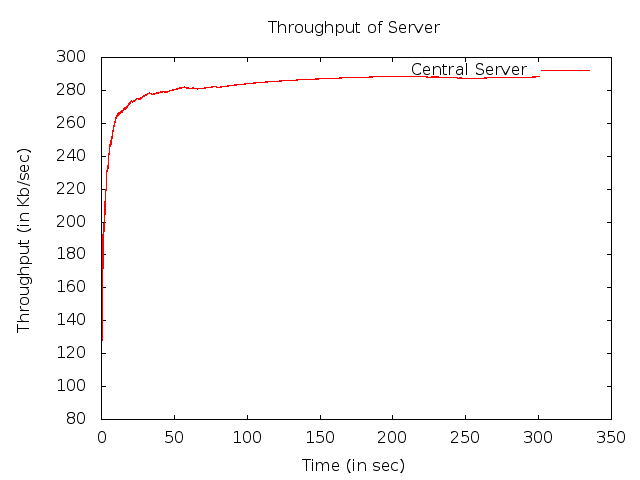
\includegraphics[width=12 cm,height=12 cm]{../problem1/throughput.png}
 % Throughput_MMK.png: 640x480 pixel, 72dpi, 22.58x16.93 cm, bb=0 0 640 480
\end{center}

\noindent Fig-6: Queue Length Vs time Graph(for M/M/1-K model)
\begin{center}
 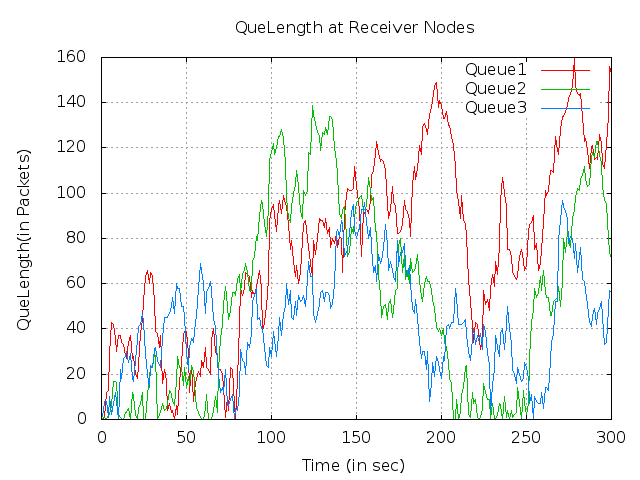
\includegraphics[width=12 cm,height=12 cm]{../problem1/queuelength.png}
 % queuelength_mmk.png: 640x480 pixel, 72dpi, 22.58x16.93 cm, bb=0 0 640 480
\end{center}
\noindent Fig-7: Interarrival Time Vs Time Graph(for M/M/1-K model )\\
\begin{center}
 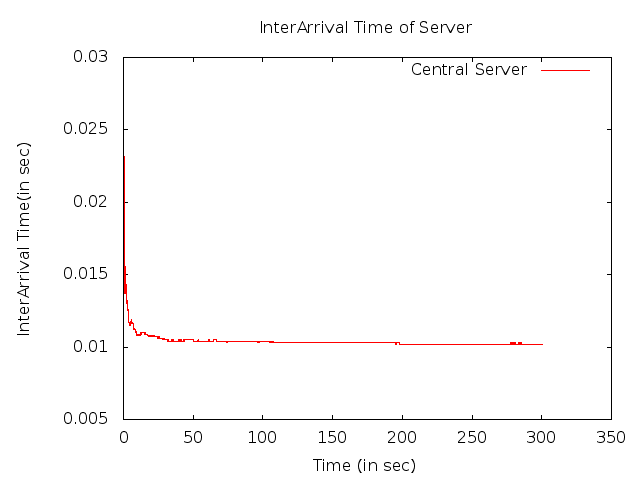
\includegraphics[width=12 cm,height=12 cm]{../problem1/interarrival.png}
 % queuelength.png: 640x480 pixel, 72dpi, 22.58x16.93 cm, bb=0 0 640 480
\end{center}
\noindent \\\\\\\\\\\\\\\\\\\\\
\noindent Fig-8: Throughput Vs time Graph(for M/D/1 model)
\begin{center}
 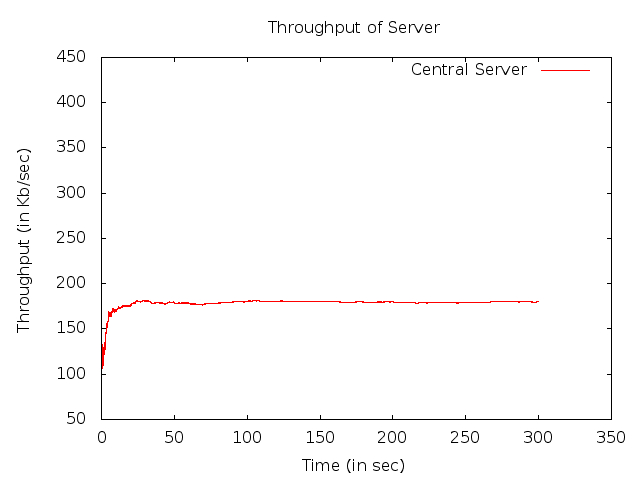
\includegraphics[width=12 cm,height=12 cm]{../problem2/throughput.png}
 % Throughput_MMK.png: 640x480 pixel, 72dpi, 22.58x16.93 cm, bb=0 0 640 480
\end{center}

\noindent Fig-9: Queue Length Vs time Graph(for M/D/1 model)
\begin{center}
 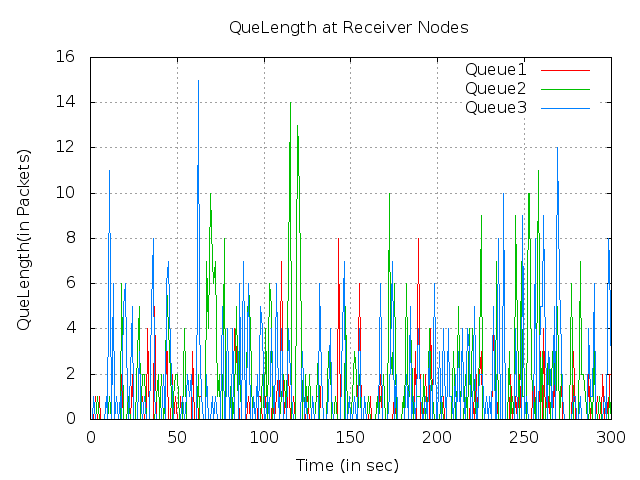
\includegraphics[width=12 cm,height=12 cm]{../problem2/queuelength.png}
 % queuelength_mmk.png: 640x480 pixel, 72dpi, 22.58x16.93 cm, bb=0 0 640 480
\end{center}
\noindent Fig-10: Interarrival Time Vs Time Graph(for M/D/1 model )\\
\begin{center}
 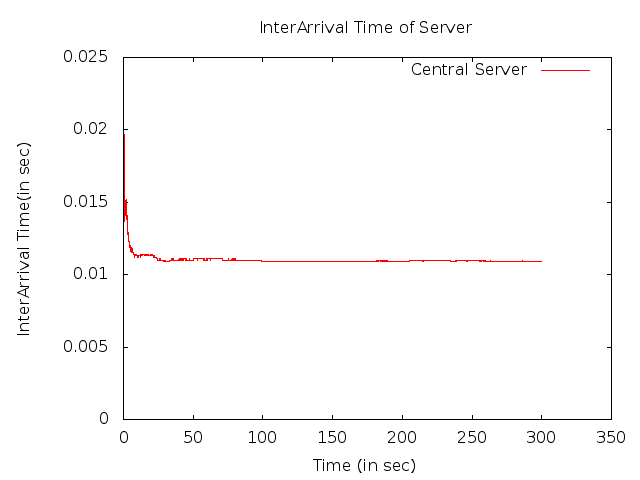
\includegraphics[width=12 cm,height=12 cm]{../problem2/interarrival.png}
 % queuelength.png: 640x480 pixel, 72dpi, 22.58x16.93 cm, bb=0 0 640 480
\end{center}



\begin{center}
\chapter{\textcolor{blue}{\underline {RESULTS AND CONCLUSIONS}}}\end{center}
\noindent The topology is designed as per the given requirements, and the simulation is working perfectly. The Graph Plotted studies the behaviour of Network under 
	  the M/M/1 and M/M/1-K queue models. As we limit the queue length to 500 for M/M/1-K model throughtput decreases as compared to the 
	  throughtput calculated for M/M/1 model.

\noindent Fig-11: Simulation Result(for M/M/1 model )\\
\begin{center}
 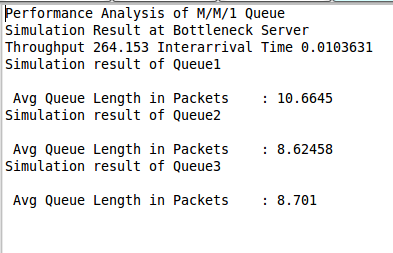
\includegraphics[width=12 cm,height=12 cm]{./result.png}
 % Throughput.png: 640x480 pixel, 72dpi, 22.58x16.93 cm, bb=0 0 640 480
\end{center}
\noindent Fig-12: Simulation Result(for M/M/1-K model )\\
\begin{center}
 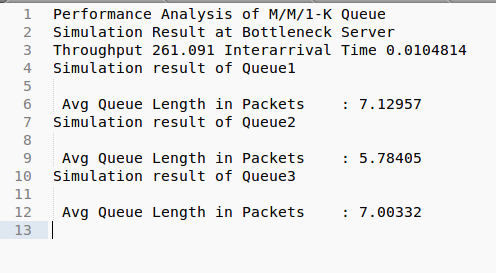
\includegraphics[width=12 cm,height=12 cm]{./result1.png}
 % Throughput.png: 640x480 pixel, 72dpi, 22.58x16.93 cm, bb=0 0 640 480
\end{center}
\noindent Fig-13: Simulation Result(for M/D/1 model )\\
\begin{center}
 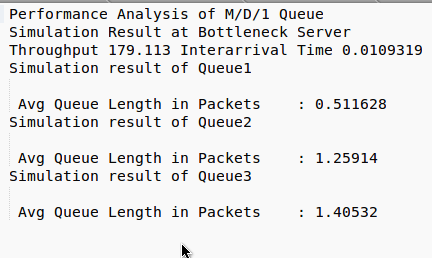
\includegraphics[width=12 cm,height=12 cm]{./result2.png}
 % Throughput.png: 640x480 pixel, 72dpi, 22.58x16.93 cm, bb=0 0 640 480
\end{center}
\end{document}  